\documentclass[a4paper,twoside]{article}

\usepackage{apalike}
\usepackage{SCITEPRESS}
\usepackage{amssymb}
\usepackage{amstext}
\usepackage{amsmath}
\usepackage{amsthm}
\usepackage{graphicx}
\usepackage{multicol}
\usepackage[small]{caption}
\usepackage{subfloat}

\usepackage{tikz}



\begin{document}


%%%%%%%%%%%%%%%%%%%%%%%%%%%%%%%%%%%%%%%%%%%%%%%%%%%%%%%%%%%%%%%%%%%%%%%%%%%%%%%%
%%%                               80 COLONNES                                %%%
%%%%%%%%%%%%%%%%%%%%%%%%%%%%%%%%%%%%%%%%%%%%%%%%%%%%%%%%%%%%%%%%%%%%%%%%%%%%%%%%


\title{Pushing the limits of Wireless Sensor Networks:
       Using 802.15.4 Radio Medium under Heavy Loads}


%\author{
%\authorname{K\'evin Roussel, Ye-Qiong Song and Olivier Zendra}
%\affiliation{LORIA/INRIA Nancy Grand-Est,\\
%             Universit\'e de Lorraine,\\
%             615, rue du Jardin Botanique,\\
%             54600 Villers-L\`es-Nancy, France}
%\email{\{Kevin.Roussel,Ye-Qiong.Song,Olivier.Zendra\}@inria.fr}
%}


\keywords{Wireless Sensor Networks, Internet of Things, Heavy Load,
          MAC protocols, ContikiMAC}


\abstract{In the literature, Wireless Sensor Networks (WSN) have been tested
and used under the assumption of light to moderate network loads. We want
to test whether they are able to perform correctly under heavy load,
trying to approach the theoretical bandwith limit of 250~kilobit/second
for the IEEE 802.15.4 radio medium.\\
As a first experiment, we tried to simulate a basic WSN, using the
reference software platform: Contiki OS and its default network stack.\\
The simulations show that this configuration can perform quite well
under heavy loads, if configuration parameters are tweaked correctly.}


\onecolumn \maketitle \normalsize \vfill

%%%%%%%%%%%%%%%%%%%%%%%%%%%%%%%%%%%%%%%%%%%%%%%%%%%%%%%%%%%%%%%%%%%%%%%%%%%%%

\section{\uppercase{Introduction}}

TODO.


%%%%%%%%%%%%%%%%%%%%%%%%%%%%%%%%%%%%%%%%%%%%%%%%%%%%%%%%%%%%%%%%%%%%%%%%%%%%%

\section{\uppercase{WSN Software platforms}}

Specialized OSes for the resource-constrained devices that constitute
wireless sensor networks have been designed, published, and made available
for quite a long time.


The first widely used system in this domain was \emph{TinyOS} \cite{TinyOS}.
It is an open-source OS, whose first stable release (1.0) was published in
september 2002. It is very lightweight, and as such well adapted to limited
devices like WSN motes.  It has brought many advances in this domain, like
the ability to use Internet Protocol (IP) and routing (RPL) on 802.15.4
networks, including the latest IPv6 version, and to simulate networks
of TinyOS motes via TOSSIM \cite{TOSSIM}.

Its main drawback is that one needs to learn a specific language---named
nesC---to be able to efficiently work within it. This language is quite
different from standard C and other common imperative programming languages,
and as such can be difficult to master.

The presence of that specific language is no coincidence: TinyOS is built
on its own specific paradigms: it has an unique stack, from which the
different components of the OS are called as statically linked callbacks.
This makes the programming of applications complex, especially for
decomposing into various ``tasks''. The multitasking part is also
quite limited: tasks are run in a fixed, queue-like order. Finally,
TinyOS requires a custom GNU-based toolchain to be built.

All of these limitations, plus a relatively slow development pace (last
stable version dates back to august 2012) have harmed its adoption,
and it is not the mainly used OS of the domain anymore.


The current reference OS in the domain of WSN and IoT is \emph{Contiki}
\cite{ContikiOS}. It's also an open-source OS, which was first released
in 2002. It is also at the origin of many assets: we can mention, among
others, the uIP Embedded TCP/IP Stack \cite{uip}, that has been extended
to uIPv6, the low-power Rime network stack \cite{Rime}, or the Cooja advanced
network simulator \cite{Cooja}.

While a bit more resource-demanding than TinyOS, Contiki is also very
lightweight and well adapted to motes. Its greatest advantage over TinyOS
is that it is based on standard, well-known OS paradigms, and coded
in standard C language, which makes it relatively easy to learn and program.
It offers an event-based kernel, implemented using cooperative multithreading,
and a complete network stack. All of these features and advantages have made
Contiki widespread, making it the reference OS when it comes to WSN.

Contiki developers also have made advances in the MAC/RDC domain: many
of them have been implemented as part of the Contiki network stack, and
a specifically developed, ContikiMAC, has been published in 2011
\cite{ContikiMAC} and implemented into Contiki as the default
RDC protocol (designed to be used with standard CSMA/CA as MAC layer).

\medskip

Consequently, we naturally decided, for our first tests, to use the Contiki
software platform: the ContikiOS, the ContikiMAC RDC protocol, the standard
CSMA/CA MAC layer, and the Rime network layer, used on the IEEE 802.15.4
physical wireless/radio protocol.


%%%%%%%%%%%%%%%%%%%%%%%%%%%%%%%%%%%%%%%%%%%%%%%%%%%%%%%%%%%%%%%%%%%%%%%%%%%%%

\section{\uppercase{Method and Benchmark}}

For our first experiments, we used, for practical reasons, the Cooja
simulator rather than actual hardware. All the simulated nodes are
virtual Zolertia Z1 motes, well-known MSP430-based devices, that are
used in real-life, industrial setups.

We have implemented test applications under Contiki OS, and made first tests
by performing simulations of a basic, but large, 802.15.4 PAN (Personal Area
Network) constituted of a ``router'', and ten motes acting as ``leaf nodes''.
The ten nodes regularly send data packets to the router, that retransmits
these data packets to a nearby ``sink'' device. Both the router and the ten
nodes use exclusively the S-CoSenS RDC/MAC protocol. This is summarized
in figure \ref{FigPANtest}.

\begin{figure}[!h]
\centering
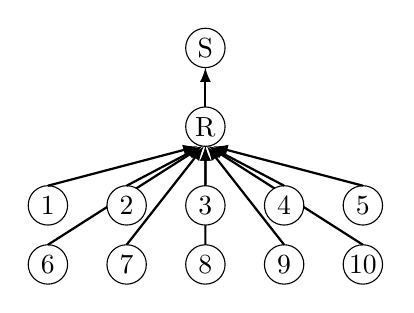
\begin{tikzpicture}[>=latex]
%sink
\draw (0, 1cm) circle (0.25cm); \draw (0, 1cm) node {S};
%router to sink link
\draw[->,thick] (0, 0.25cm) -- (0, 0.75cm);
%router
\draw (0, 0) circle (0.25cm); \draw (0, 0) node {R};
%leaf nodes (lower)
\foreach \x in {6,7,8,9,10}
{
  \fill[white] (\x * 1cm - 8cm, -1.75cm) circle (0.25cm);
  \draw (\x * 1cm - 8cm, -1.75cm) circle (0.25cm);
  \draw (\x * 1cm - 8cm, -1.75cm) node {\x};
  % link to router
  \draw[->,thick] (\x * 1cm - 8cm, -1.5cm)
                  -- (\x * 0.02cm - 0.16cm, -0.25cm);
}
%leaf nodes (upper)
\foreach \x in {1,2,3,4,5}
{
  \fill[white] (\x * 1cm - 3cm, -1cm) circle (0.25cm);
  \draw (\x * 1cm - 3cm, -1cm) circle (0.25cm);
  \draw (\x * 1cm - 3cm, -1cm) node {\x};
  % link to router
  \draw[->,thick] (\x * 1cm - 3cm, -0.75cm)
                  -- (\x * 0.05cm - 0.15cm, -0.25cm);
}
\end{tikzpicture}
\caption{Functional schema of our virtual test PAN.}
\label{FigPANtest}
\end{figure}

We then performed simulations on this virtual PAN, varying several parameters
of the ContikiMAC RDC protocol, under moderately-heavy to extreme network
loads. The loads were generated by the application loaded on the 10 leaf
nodes: they were programmed to generate large 802.15.4 network packets
(90 bytes of payload, which translates to an actual packet size of
around 110 bytes) at a fixed rate, with random variations to avoid
medium congestion. The different setups are described in table
\ref{TblDataRates}: the table gives the average delay between
each packet transmission on each mote, the average number of
packets emitted every second for the 10 nodes, and the expected
resulting data rate.

\begin{table}[htb]
\centering
\begin{tabular}{|l|r|r|r|}
\hline
Setup     &  Delay  & Pkts/s & Data Rate \\
\hline
Moderate  & 1500 ms &   6.7  &  5,867 bit/s \\ 
High      & 1000 ms &  10    &  8,800 bit/s \\
Very High &  500 ms &  20    & 17,600 bit/s \\
Extreme   &  100 ms & 100    & 88,000 bit/s \\
\hline
\end{tabular}
\caption{Transmission data rates used on leaf nodes.}
\label{TblDataRates}
\end{table}

For each scenario, we performed two kind of simulations:
\begin{itemize}
\item a \emph{fixed packet number simulation}, during which each node emits
500 packets at the fixed rate, then turns off; the simulation ends when all
nodes have transmitted their quota of packets;

\item a \emph{fixed duration simulation}, during which each node emits an
unspecified number of packets at the fixed rate; the simultaion ends after
10 minutes.
\end{itemize}

These diffrent kind of simulations allow us to easily determine respectively
QoS and duty cycle statistics without bias, as we will now see in the next
section.


%%%%%%%%%%%%%%%%%%%%%%%%%%%%%%%%%%%%%%%%%%%%%%%%%%%%%%%%%%%%%%%%%%%%%%%%%%%%%

\section{\uppercase{Results and Discussion}}

\subsection{Quality of Service (QoS)}

We quantify the QoS, in our simulations of WSN, by the number of packets
that arrive to their destination, that is: the number of packets that are
sent from one of the leaf nodes, relayed by the router, and are actually
received by the sink.

Using the \emph{fixed packet number simulations}, we can easily compute the
rate of packets that arrive to destination, compared to the known number
of packets emitted by the nodes.

Thus, we were able to determine that the only parameter that has actually
influence on the QoS is the rate at which the ContikiMAC RDC protocol
senses the radio medium. This parameter is named
\texttt{NETSTACK\_CONF\_RDC\_CHANNEL\_CHECK\_RATE} in Contiki source code.
Its default value is 8, meaning the radio channel is checked eight times
per second; this parameter is actually given in Hertz.

Note we also allowed the the standard CSMA/CA MAC layer to perform up to
seven retries for a given data packet, by setting the
\texttt{CSMA\_CONF\_MAX\_MAC\_TRANSMISSIONS}
parameter to 8 in Contiki source code.

This default value of 8~Hz only gives poor results concerning QoS.
We changed the parameter value, and doubled it up to 256~Hz. The results
we obtained are shown in table \ref{TblSuccessRate}.

\begin{table*}[htbp]
\centering
\begin{tabular}{|r|r|r|r|r|}
\hline
Setup & Moderate & High & Very High & Extreme \\
\hline
\multicolumn{5}{|l|}{Channel Check Rate = 8 Hz}\\
\hline
NODES & & & & \\
packets lost & 121 & 190 & 1086 & 3190 \\
packets transmitted & 4879 & 4810 & 3914 & 1810 \\
success rate & 97.58\% & 96.20\% & 78.28\% & 36.20\% \\
ROUTER & & & & \\
packets lost & 2394 & 3167 & 3194 & 1778 \\
packets transmitted & 2485 & 1641 & 722 & 32 \\
success rate & 49.70\% & 32.82\% & 14.44\% & 0.64\% \\
\hline
\multicolumn{5}{|l|}{Channel Check Rate = 16 Hz}\\
\hline
NODES & & & & \\
packets lost & 14 & 48 & 173 & 2532 \\
packets transmitted & 4986 & 4952 & 4827 & 2468 \\
success rate & 99.72\% & 99.04\% & 96.54\% & 49.36\% \\
ROUTER & & & & \\
packets lost & 39 & 1029 & 3724 & 2042 \\
packets transmitted & 4947 & 3922 & 1106 & 434 \\
success rate & 98.94\% & 78.44\% & 22.12\% & 8.68\% \\
\hline
\multicolumn{5}{|l|}{Channel Check Rate = 32 Hz}\\
\hline
NODES & & & & \\
packets lost & 0 & 3 & 41 & 1668 \\
packets transmitted & 5000 & 4997 & 4959 & 3332 \\
success rate & 100\% & 99.94\% & 99.18\% & 66.64\% \\
ROUTER & & & & \\
packets lost & 0 & 0 & 641 & 3048 \\
packets transmitted & 5000 & 4996 & 4316 & 299 \\
success rate & 100\% & 99.92\% & 86.32\% & 5.98\% \\
\hline
\multicolumn{5}{|l|}{Channel Check Rate = 64 Hz}\\
\hline
NODES & & & & \\
packets lost & & & & \\
packets transmitted & & & & \\
success rate & \% & \% & \% & \% \\
ROUTER & & & & \\
packets lost & & & & \\
packets transmitted & & & & \\
success rate & \% & \% & \% & \% \\
\hline
\multicolumn{5}{|l|}{Channel Check Rate = 128 Hz}\\
\hline
NODES & & & & \\
packets lost & & & & \\
packets transmitted & & & & \\
success rate & \% & \% & \% & \% \\
ROUTER & & & & \\
packets lost & & & & \\
packets transmitted & & & & \\
success rate & \% & \% & \% & \% \\
\hline
\multicolumn{5}{|l|}{Channel Check Rate = 256 Hz}\\
\hline
NODES & & & & \\
packets lost & & & & \\
packets transmitted & & & & \\
success rate & \% & \% & \% & \% \\
ROUTER & & & & \\
packets lost & & & & \\
packets transmitted & & & & \\
success rate & \% & \% & \% & \% \\
\hline
Setup & Moderate & High & Very High & Extreme \\
\hline
\end{tabular}
\caption{Rate of packets arrived to their destination,
         according to the ContikiMAC channel check rate.\\
         Results obtained with fixed packet number simulations.}
\label{TblSuccessRate}
\end{table*}

The data shown in table \ref{TblSuccessRate} shows us many facts:

\begin{itemize}

\item \emph{The QoS increases with Channel Check Rate.} While the default
rate of 8~Hz gives poor results in every case, each doubling of frequency
allows us to obtain excellent results (destination arrival rate of 98\%
or more) in a new scenario. At 128~Hz, we get an acceptable rate (nn\%)
even in the extreme setup.

\item \emph{The packet losses are mainly due to the router.}\\
In the ``moderate'' and ``high'' setups, communication between the nodes
and their router is always satisfactory (success rate of 95\% and more):
all packet losses are due to the router being unable to relay the packets
it receives to the sink.\\
In the ``very high'' setup, the situation is identical at frequencies
of 16~Hz and more; at the default frequency of 8~Hz: communication between
nodes and router is less satifactory (only 78\% of success), but the vast
majority of packet loss (about 64\% of all the emitted packets) is still
due to the router.\\
In the ``extreme'' setup, there are major losses at the node level at 8~Hz
and 16~Hz, but at 32~Hz and more, the packet losses are again mainly due
to the router.\\
We can then conclude that relaying packets at the router level is the
weak point of the software platform, and more precisely of the ContikiMAC
RDC protocol.

\item \emph{The network transmission stalls at a channel check frequency
of 256~Hz.} All results drop dramatically at that frequency.
This is easily explained: a channel frequency of 256~Hz only leaves
4~milliseconds of duty cycle, while a 110 byte packet to be transmitted
physically needs 3.5~ms to be transferred on the physical radio medium
(at the IEEE 802.15.4 standard rate of 250~kbit/s). This frequency is
thus saturating the physical medium. We can then easily conclude that
using a channel check frequency of 256~Hz or more is counter-productive,
and can only give unsatisfactory results.\\
\emph{We would then recommend 128~Hz as the maximal value for the channel
check frequency parameter.}

\end{itemize}

To sum it up, we see that increasing (doubling) the channel check frequency
of the ContikiMAC RDC protocol does increase the QoS of the underlying WSN,
up to and including a frequency of 128~Hz.

%%%%%%%%%%%%%%%%%%%%%%%%%%%%%%%%%%%%%%%%%%%%%%%%%%%%%%%%%%%%%%%%%%%%%%%%%%%%%

\subsection{Duty Cycle Statistics}

We also interested in the duty cycle statistics, that the Cooja simulator
can automatically calculate thanks to its timeline plugin. These values,
which indicate how much proportion of the (simulation) time the radio
transceivers of the motes are online, actually transmitting and receiving
packets and interferences, are a good indicator of the energy wasted or
spared by the system. In a WSN mote, the radio transceiver is indeed the
most energy-consuming part, well before the central microcontroller and
the various physical sensors.

For these statistics, we will use the data we collected using the
\emph{fixed duration simulations}: they allow us to maintain a regular
network activity level during a 10-minute span common to all our scenarios.

The duty cycle statistics we collected thanks to these simulations are
presented in tables \ref{TblDutyCycleStatsA} and \ref{TblDutyCycleStatsB}.

\begin{subtables}
\begin{table*}[htbp]
\centering
\begin{tabular}{|r|r|r|r|r|}
\hline
Setup & Moderate & High & Very High & Extreme \\
\hline
\multicolumn{5}{|l|}{Channel Check Rate = 8 Hz}\\
\hline
NODES (average) & & & & \\
Radio Transceiver Active & 3.38\% & 3.87\% & 4.79\% & 6.11\% \\
Packet Transmission & 1.42\% & 1.65\% & 2.21\% & 2.93\% \\
Packet Reception & 0.19\% & 0.22\% & 0.26\% & 0.40\% \\
Interference Reception & 0.15\% & 0.18\% & 0.23\% & 0.24\% \\
ROUTER & & & & \\
Radio Transceiver Active & 8.62\% & 11.12\% & 14.98\% & 26.99\% \\
Packet Transmission & 1.35\% & 1.50\% & 1.33\% & 1.38\% \\
Packet Reception & 2.55\% & 3.66\% & 5.77\% & 12.33\% \\
Interference Reception & 0.93\% & 1.27\% & 1.61\% & 1.58\% \\
\hline
\multicolumn{5}{|l|}{Channel Check Rate = 16 Hz}\\
\hline
NODES (average) & & & & \\
Radio Transceiver Active & 4.16\% & 6.56\% & 8.80\% & 10.69\% \\
Packet Transmission & 1.11\% & 2.15\% & 3.21\% & 4.22\% \\
Packet Reception & 0.47\% & 0.70\% & 0.82\% & 0.99\% \\
Interference Reception & 0.14\% & 0.43\% & 0.75\% & 0.85\% \\
ROUTER & & & & \\
Radio Transceiver Active & 11.55\% & 15.41\% & 21.12\% & 42.53\% \\
Packet Transmission & 2.60\% & 3.22\% & 2.25\% & 8.91\% \\
Packet Reception & 2.74\% & 4.05\% & 7.30\% & 17.87\% \\
Interference Reception & 0.39\% & 1.26\% & 2.59\% & 3.68\% \\
\hline
\multicolumn{5}{|l|}{Channel Check Rate = 32 Hz}\\
\hline
NODES (average) & & & & \\
Radio Transceiver Active & 5.61\% & 7.45\% & 14.27\% & 18.20\% \\
Packet Transmission & 0.90\% & 1.48\% & 3.89\% & 5.54\% \\
Packet Reception & 0.66\% & 1.03\% & 1.96\% & 2.32\% \\
Interference Reception & 0.11\% & 0.21\% & 1.13\% & 1.63\% \\
ROUTER & & & & \\
Radio Transceiver Active & 12.77\% & 17.85\% & 31.13\% & 58.76\% \\
Packet Transmission & 2.64\% & 4.00\% & 6.88\% & 4.16\% \\
Packet Reception & 2.78\% & 4.18\% & 8.24\% & 23.02\% \\
Interference Reception & 0.16\% & 0.40\% & 2.64\% & 6.64\% \\
\hline
Setup & Moderate & High & Very High & Extreme \\
\hline
\end{tabular}
\caption{Duty cycle statistics, according to the ContikiMAC channel
         check rate (8 to 32 Hz).\\
         Results obtained with fixed 10-minute duration simulations.}
\label{TblDutyCycleStatsA}
\end{table*}

\begin{table*}[htbp]
\centering
\begin{tabular}{|r|r|r|r|r|}
\hline
Setup & Moderate & High & Very High & Extreme \\
\hline
\multicolumn{5}{|l|}{Channel Check Rate = 64 Hz}\\
\hline
NODES (average) & & & & \\
Radio Transceiver Active & 10.11\% & 12.81\% & 24.41\% & 29.95\% \\
Packet Transmission & 0.76\% & 1.25\% & 3.70\% & 5.64\% \\
Packet Reception & 1.24\% & 1.95\% & 4.62\% & 4.13\% \\
Interference Reception & 0.53\% & 0.29\% & 2.03\% & 3.93\% \\
ROUTER & & & & \\
Radio Transceiver Active & 15.38\% & 20.61\% & 39.33\% & 71.99\% \\
Packet Transmission & 2.70\% & 4.06\% & 9.07\% & 8.32\% \\
Packet Reception & 2.76\% & 4.19\% & 8.95\% & 24.77\% \\
Interference Reception & 0.07\% & 0.17\% & 1.98\% & 10.45\% \\
\hline
\multicolumn{5}{|l|}{Channel Check Rate = 128 Hz}\\
\hline
NODES (average) & & & & \\
Radio Transceiver Active & 18.69\% & 23.72\% & 47.51\% & 43.52\% \\
Packet Transmission & 0.82\% & 1.39\% & 5.97\% & 5.15\% \\
Packet Reception & 2.42\% & 3.84\% & 6.53\% & 4.91\% \\
Interference Reception & 0.38\% & 0.76\% & 7.10\% & 5.10\% \\
ROUTER & & & & \\
Radio Transceiver Active & 21.02\% & 26.93\% & 51.24\% & 67.15\% \\
Packet Transmission & 2.71\% & 4.18\% & 7.82\% & 12.29\% \\
Packet Reception & 2.98\% & 4.46\% & 8.27\% & 16.63\% \\
Interference Reception & 0.20\% & 0.46\% & 6.78\% & 5.88\% \\
\hline
\multicolumn{5}{|l|}{Channel Check Rate = 256 Hz}\\
\hline
NODES (average) & & & & \\
Radio Transceiver Active & 21.30\% & 21.33\% & 21.32\% & 21.31\% \\
Packet Transmission & 0.02\% & 0.02\% & 0.02\% & 0.02\% \\
Packet Reception & 0.05\% & 0.06\% & 0.05\% & 0.05\% \\
Interference Reception & 0.00\% & 0.00\% & 0.00\% & 0.00\% \\
ROUTER & & & & \\
Radio Transceiver Active & 21.43\% & 21.43\% & 21.48\% & 21.46\% \\
Packet Transmission & 0.03\% & 0.03\% & 0.03\% & 0.03\% \\
Packet Reception & 0.16\% & 0.16\% & 0.19\% & 0.17\% \\
Interference Reception & 0.00\% & 0.00\% & 0.00\% & 0.00\% \\
\hline
\end{tabular}
\caption{Duty cycle statistics, according to the ContikiMAC channel
         check rate (64 to 256 Hz).\\
         Results obtained with fixed 10-minute duration simulations.}
\label{TblDutyCycleStatsB}
\end{table*}
\end{subtables}

The data shown in tables \ref{TblDutyCycleStatsA} and \ref{TblDutyCycleStatsB}
shows that:

\begin{itemize}

\item \emph{Duty cycle statistics also stall at a channel check frequency
of 256~Hz}. It confirms the QoS data, proving that a frequency of 256~Hz
or more is not a viable option. Again, \emph{the maximal usable value
for channel check frequency is indeed 128~Hz.}

\item \emph{Radio Transceiver Activation Rate is high: we are no more
in the low power consumption domain.} The transceiver activation rate
is always much higher than 1\% in every setup, for any frequency, for
the leaf nodes as well as for the router, meaning the very-low-power
consumption feature of ContikiMAC is irremediably lost.\\
For high channel check frequencies (64~Hz and more), as well as for
``high'' setup and heavier duty loads, transceiver activation rate
also goes (far) beyond 10\%, especially for leaf nodes, meaning that
even looking for ``basic'' low-power consumption is impossible.
Radio duty cycles, under such pressure, quickly go into the high
and very-high domain.\\
One of the major characteristics and advantages of ContikiMAC---being
very-low- or even low-power friendly--- is thus lost, when running
in the situations we want to study.

\item \emph{Duty cycle statistics---logically---raise with the rate of
exchanged data on the network medium.} Nothing surprising here.

\item \emph{Duty cycle statistics---logically---raise with the channel check
frequency}, up to the limit of 128~Hz explained hereabove.

\end{itemize}

From the last two facts, we can then recommend, for a given setup
(i.e.: a given data rate on the radio medium) to use the lowest channel
check frequency that allows to obtain the desired QoS level.
For example, it would be 16~Hz for our ``moderate'' setup, 32~Hz for
``high'', and 64~Hz for ``very high''.

As an exception, we note that at 128~Hz, the nodes' statistics for the
``extreme'' setup go down both from the 64~Hz frequency and the ``very high''
setup. We think this is simply due to the saturation of the radio medium
bandwith between the router and its leaf nodes.

To sum it up, we see that duty cycle statistics do agree with conclusions
that one would have instinctively done about the influence of channel check
frequency and network bandwith use on radio transceiver activity---and thus,
on energy consumption.

%%%%%%%%%%%%%%%%%%%%%%%%%%%%%%%%%%%%%%%%%%%%%%%%%%%%%%%%%%%%%%%%%%%%%%%%%%%%%

\subsection{Limitations and Inconsistencies}
\label{SectLimits}

The current work has of course its limitations:

\begin{itemize}

\item \emph{Those are only simulations.} To be truly accurate, we would need
to run these tests on actual hardware.\\
Moreover, we constated, during our simulations, an anomaly in the MSPSim
software (the MSP430 device simulator used by Cooja to emulate MSP430-based
motes at the cycle level \cite{MSPSim}): \emph{the delay used by the
simulator to load our large---around 110 bytes---IEEE 802.15.4 packets into
the CC2420 transceiver TX buffer is too long;} it takes around 3~milliseconds
to load such a packet to the transceiver in simulation, while our tests
on the real Zolertia Z1 hardware have explicitely and undoubtly shown that
loading times are actually about 1~millisecond long. We didn't have time
to investigate the problem and correct that anomaly.\\
We also don't know whether or not there are other inconsistencies in
the simulator software that could also alter the results of our
simulations...\\
Such anomalies will probably change the results obtained on real
hardware using the same scenarii and parameters. Unfortunately, we don't
have enough Z1 motes nor time to perform these real-life tests yet.

\item \emph{We didn't have time to study other results.} We especially
didn't have time to study radio traces to determine the transmission
delay of packets from leaf nodes up to their destination (sink).

\end{itemize}

However, we firmly believe that the general facts we observed in our
simulations won't be overturned by these problems. That's why we still
present them in the current article.


%%%%%%%%%%%%%%%%%%%%%%%%%%%%%%%%%%%%%%%%%%%%%%%%%%%%%%%%%%%%%%%%%%%%%%%%%%%%%

\section{\uppercase{Conclusion and Future Works}}

We have build simulation scenarios to test whether the current reference
sofware platform for WSN---Contiki OS, ContikiMAC, Rime network
stack---could handle heavy loads, trying to approach the theoretical
limit of 250~kbit/s of bandwith for the underlying IEEE 802.15.4
radio medium.

We were able to show---with the limits and preventions discussed hereabove
in section \ref{SectLimits}---that this reference software platform, while
designed for much lighter network loads, can handle quite gracefully the
heavy loads we imposed on it during our simulations, managing to obtain
a good to excellent QoS (few packets lost during transmissions).

To that end, however, one has to change parameters in the Contiki source
code, especially the channel check frequency, the default value for these
parameters being totally unfit to handle the heavy loads in an acceptable
manner.

One must also accept that there is no way to keep the very low power
consumption feature when dealing with such heavy network loads, the
motes' radio transceivers being heavily activated and solicited to
handle that charge.

\medskip

In the future, we would like to try other software platforms with the same
scenarii, especially by using different MAC and RDC layers in the network
stacks, and different operating systems. We may also try to use different,
new hardware devices to run our tests.

We hope to find a way to get a similar or better QoS than the one we observed
here, while trying to optimize duty cycle statistics to minimize the energy
consumption when running WSN under heavy network loads.


%%%%%%%%%%%%%%%%%%%%%%%%%%%%%%%%%%%%%%%%%%%%%%%%%%%%%%%%%%%%%%%%%%%%%%%%%%%%%


\vfill
\bibliographystyle{apalike}
{\small
\bibliography{peccs2015}}


\end{document}
